\chapter{NỀN TẢNG LÝ THUYẾT}

\section{Hệ thống khuyến nghị (Recommender Systems)}

Hệ thống khuyến nghị là một dạng của hệ thống lọc thông tin (Information Filtering), có nhiệm vụ dự đoán sự quan tâm hoặc xếp hạng của người dùng đối với một tập hợp các sản phẩm hoặc dịch vụ. Trong kỷ nguyên kinh tế số, hệ thống này đóng vai trò là cầu nối quan trọng giữa khối lượng dữ liệu khổng lồ và nhu cầu cụ thể của từng cá nhân, giúp giảm thiểu hiện tượng quá tải thông tin và tối ưu hóa doanh thu cho các nền tảng thương mại điện tử, mạng xã hội và dịch vụ giải trí.

Về cơ bản, các phương pháp xây dựng hệ thống khuyến nghị được phân loại thành ba nhóm kỹ thuật chính:

\begin{itemize}
    \item \textbf{Lọc dựa trên nội dung (Content-Based Filtering):} Phương pháp này đưa ra các gợi ý dựa trên sự tương đồng về thuộc tính của sản phẩm (như mô tả văn bản, danh mục, giá cả) với các sản phẩm mà người dùng đã tương tác trong quá khứ. Ưu điểm của phương pháp này là có thể giải quyết tốt bài toán người dùng mới (nếu họ đã thể hiện sở thích cụ thể), nhưng lại bị giới hạn bởi khả năng khám phá các sở thích mới bên ngoài các thuộc tính đã biết.
    \item \textbf{Lọc cộng tác (Collaborative Filtering - CF):} Đây là phương pháp phổ biến nhất, dựa trên giả thuyết rằng những người dùng có hành vi tương tự trong quá khứ sẽ có xu hướng quan tâm đến các sản phẩm giống nhau trong tương lai. CF bao gồm hai hướng tiếp cận chính là dựa trên láng giềng (kNN) và dựa trên mô hình (Matrix Factorization). Mặc dù hiệu quả, CF thường đối mặt với các thách thức lớn như dữ liệu thưa thớt (Sparsity) và bài toán người dùng/sản phẩm mới hoàn toàn (Cold-start).
    \item \textbf{Phương pháp lai (Hybrid Methods):} Kết hợp các đặc tính ưu việt của cả lọc nội dung và lọc cộng tác nhằm khắc phục nhược điểm của từng phương pháp riêng lẻ, từ đó nâng cao độ chính xác và tính ổn định của hệ thống.
\end{itemize}

Mặc dù đã đạt được nhiều thành công, các hệ thống khuyến nghị truyền thống vẫn tồn tại những hạn chế cố hữu. Cụ thể, các mô hình Matrix Factorization thường khó mô hình hóa được các mối quan hệ phi tuyến tính phức tạp giữa người dùng và sản phẩm. Bên cạnh đó, việc dữ liệu bị thưa thớt khiến các phương pháp dựa trên sự tương đồng trực tiếp không đạt được hiệu suất tối ưu. Những thách thức này đã thúc đẩy việc ứng dụng Deep Learning và đặc biệt là Mạng nơ-ron đồ thị (Graph Neural Networks) để khai thác sâu hơn cấu trúc liên kết giữa các thực thể trong không gian dữ liệu.

\section{Graph Neural Networks (GNN)}

Mạng nơ-ron đồ thị (Graph Neural Networks - GNN) là một lớp kiến trúc học sâu được thiết kế để xử lý dữ liệu có cấu trúc đồ thị. Khác với các mạng nơ-ron truyền thống như CNN hay RNN vốn hoạt động trên dữ liệu có cấu trúc lưới (grid) hoặc chuỗi (sequence), GNN cho phép khai thác thông tin từ các mối quan hệ phức tạp và phi cấu trúc giữa các thực thể.

\subsection{Định nghĩa đồ thị (Graph)}

Một đồ thị $\mathcal{G}$ được định nghĩa bởi một bộ $(\mathcal{V}, \mathcal{E})$, trong đó $\mathcal{V}$ là tập hợp các nút (nodes) và $\mathcal{E}$ là tập hợp các cạnh (edges) biểu diễn mối quan hệ giữa các nút.
\begin{itemize}
    \item \textbf{Ma trận kề (Adjacency Matrix - $A$):} Biểu diễn cấu trúc kết nối của đồ thị, trong đó $A_{ij} = 1$ nếu có cạnh nối giữa nút $i$ và nút $j$, ngược lại $A_{ij} = 0$.
    \item \textbf{Ma trận đặc trưng nút (Node Feature Matrix - $X$):} Mỗi nút $v \in \mathcal{V}$ được gán một vector đặc trưng $x_v \in \mathbb{R}^d$, biểu diễn các thuộc tính của nút đó.
    \item \textbf{Đồ thị dị nhất (Heterogeneous Graph):} Là đồ thị chứa nhiều loại nút và nhiều loại cạnh khác nhau. Đây là cấu trúc được sử dụng trong đề tài để biểu diễn các thực thể như người dùng (User) và sản phẩm (Item) cùng các tương tác đa dạng giữa chúng.
\end{itemize}

\subsection{Cơ chế Message Passing}

Hầu hết các kiến trúc GNN hiện đại đều dựa trên cơ chế truyền thông điệp (Message Passing). Ý tưởng cốt lõi là trạng thái của một nút sẽ được cập nhật liên tục thông qua việc tổng hợp thông tin từ các nút láng giềng trực tiếp của nó. Quá trình này tại tầng $k$ được mô tả qua hai bước chính:

\begin{enumerate}
    \item \textbf{Tổng hợp (Aggregation):} Thu thập các vector đặc trưng từ các nút láng giềng $\mathcal{N}(v)$.
    \item \textbf{Cập nhật (Update):} Kết hợp thông tin đã tổng hợp được với đặc trưng hiện tại của nút $v$ để tạo ra vector biểu diễn mới $h_v^{(k)}$.
\end{enumerate}

Công thức tổng quát của cơ chế này như sau:
\begin{equation}
    h_v^{(k)} = \text{UPDATE}^{(k)} \left( h_v^{(k-1)}, \text{AGGREGATE}^{(k)} \left( \{ h_u^{(k-1)} : u \in \mathcal{N}(v) \} \right) \right)
\end{equation}

Sau $K$ tầng lan truyền, mỗi nút sẽ sở hữu một vector nhúng (embedding) chứa đựng thông tin về cấu trúc và đặc trưng của vùng lân cận $K$-hop xung quanh nó.

\subsection{Các biến thể GNN tiêu biểu}

Sự khác biệt giữa các kiến trúc GNN chủ yếu nằm ở cách thiết kế hàm \textit{AGGREGATE} và \textit{UPDATE}:

\begin{itemize}
    \item \textbf{GCN (Graph Convolutional Network):} Sử dụng hàm tổng hợp trung bình có trọng số dựa trên bậc của các nút, giúp chuẩn hóa thông tin trong quá trình lan truyền.
    \item \textbf{GAT (Graph Attention Network):} Áp dụng cơ chế chú ý (Attention Mechanism) để gán các trọng số khác nhau cho các láng giềng khác nhau, cho phép mô hình tập trung vào các thông tin quan trọng hơn.
    \item \textbf{GraphSAGE (Graph Sample and AggregatE):} Thay vì sử dụng toàn bộ láng giềng, GraphSAGE thực hiện lấy mẫu một số lượng cố định láng giềng. Điều này không chỉ giúp giảm chi phí tính toán mà còn giúp mô hình có khả năng học quy nạp (inductive), cho phép sinh vector nhúng cho các nút chưa từng xuất hiện trong quá trình huấn luyện. Đây là mô hình cốt lõi được lựa chọn để hiện thực hóa hệ thống khuyến nghị trong đề tài này.
\end{itemize}

\section{GraphSAGE}

GraphSAGE (Graph Sample and AggregatE) là một framework học biểu diễn đồ thị mang tính quy nạp (inductive), cho phép sinh ra các vector nhúng cho các nút chưa từng xuất hiện trong tập huấn luyện bằng cách khai thác các đặc trưng nút và cấu trúc lân cận cục bộ. Đây là một bước tiến quan trọng so với các phương pháp truyền thống vốn mang tính xuyên nạp (transductive), đòi hỏi tất cả các nút phải hiện diện trong đồ thị tại thời điểm huấn luyện.

\subsection{Ý tưởng cốt lõi và Tính quy nạp}

Thay vì học một vector nhúng cố định cho từng nút, GraphSAGE tập trung vào việc học một tập hợp các hàm tổng hợp (aggregator functions). Khi gặp một nút mới, mô hình chỉ cần áp dụng các hàm này lên các đặc trưng của nút đó và các láng giềng xung quanh để tạo ra vector biểu diễn. Khả năng này cực kỳ quan trọng trong các hệ thống khuyến nghị thực tế, nơi các sản phẩm và người dùng mới liên tục được thêm vào hệ thống.

\subsection{Quy trình lan truyền và tổng hợp}

Quy trình sinh vector biểu diễn của GraphSAGE tại mỗi tầng $k$ bao gồm ba bước chính:

\begin{enumerate}
    \item \textbf{Lấy mẫu láng giềng (Neighbor Sampling):} Để giải quyết vấn đề bùng nổ tính toán trên các đồ thị lớn, GraphSAGE lấy mẫu một số lượng cố định láng giềng $\mathcal{N}(v)$ cho mỗi nút thay vì sử dụng toàn bộ tập láng giềng.
    \item \textbf{Tổng hợp đặc trưng (Aggregation):} Các đặc trưng từ các láng giềng được tổng hợp lại thành một vector duy nhất thông qua hàm $AGGREGATE_k$.
    \item \textbf{Kết hợp và Cập nhật (Combine \& Update):} Vector tổng hợp từ láng giềng được nối (concatenate) với vector đặc trưng hiện tại của nút $v$, sau đó đi qua một biến đổi tuyến tính và hàm kích hoạt phi tuyến $\sigma$ (thường là ReLU).
\end{enumerate}

Công thức toán học cụ thể:
\begin{equation}
    h_{\mathcal{N}(v)}^{(k)} = \text{AGGREGATE}_k \left( \{ h_u^{(k-1)}, \forall u \in \mathcal{N}(v) \} \right)
\end{equation}
\begin{equation}
    h_v^{(k)} = \sigma \left( W^{(k)} \cdot \text{CONCAT} \left( h_v^{(k-1)}, h_{\mathcal{N}(v)}^{(k)} \right) \right)
\end{equation}

Sau bước này, vector $h_v^{(k)}$ thường được chuẩn hóa về độ dài đơn vị (L2 normalization) để đảm bảo tính ổn định trong quá trình huấn luyện.

\begin{figure}[htbp]
    \centering
    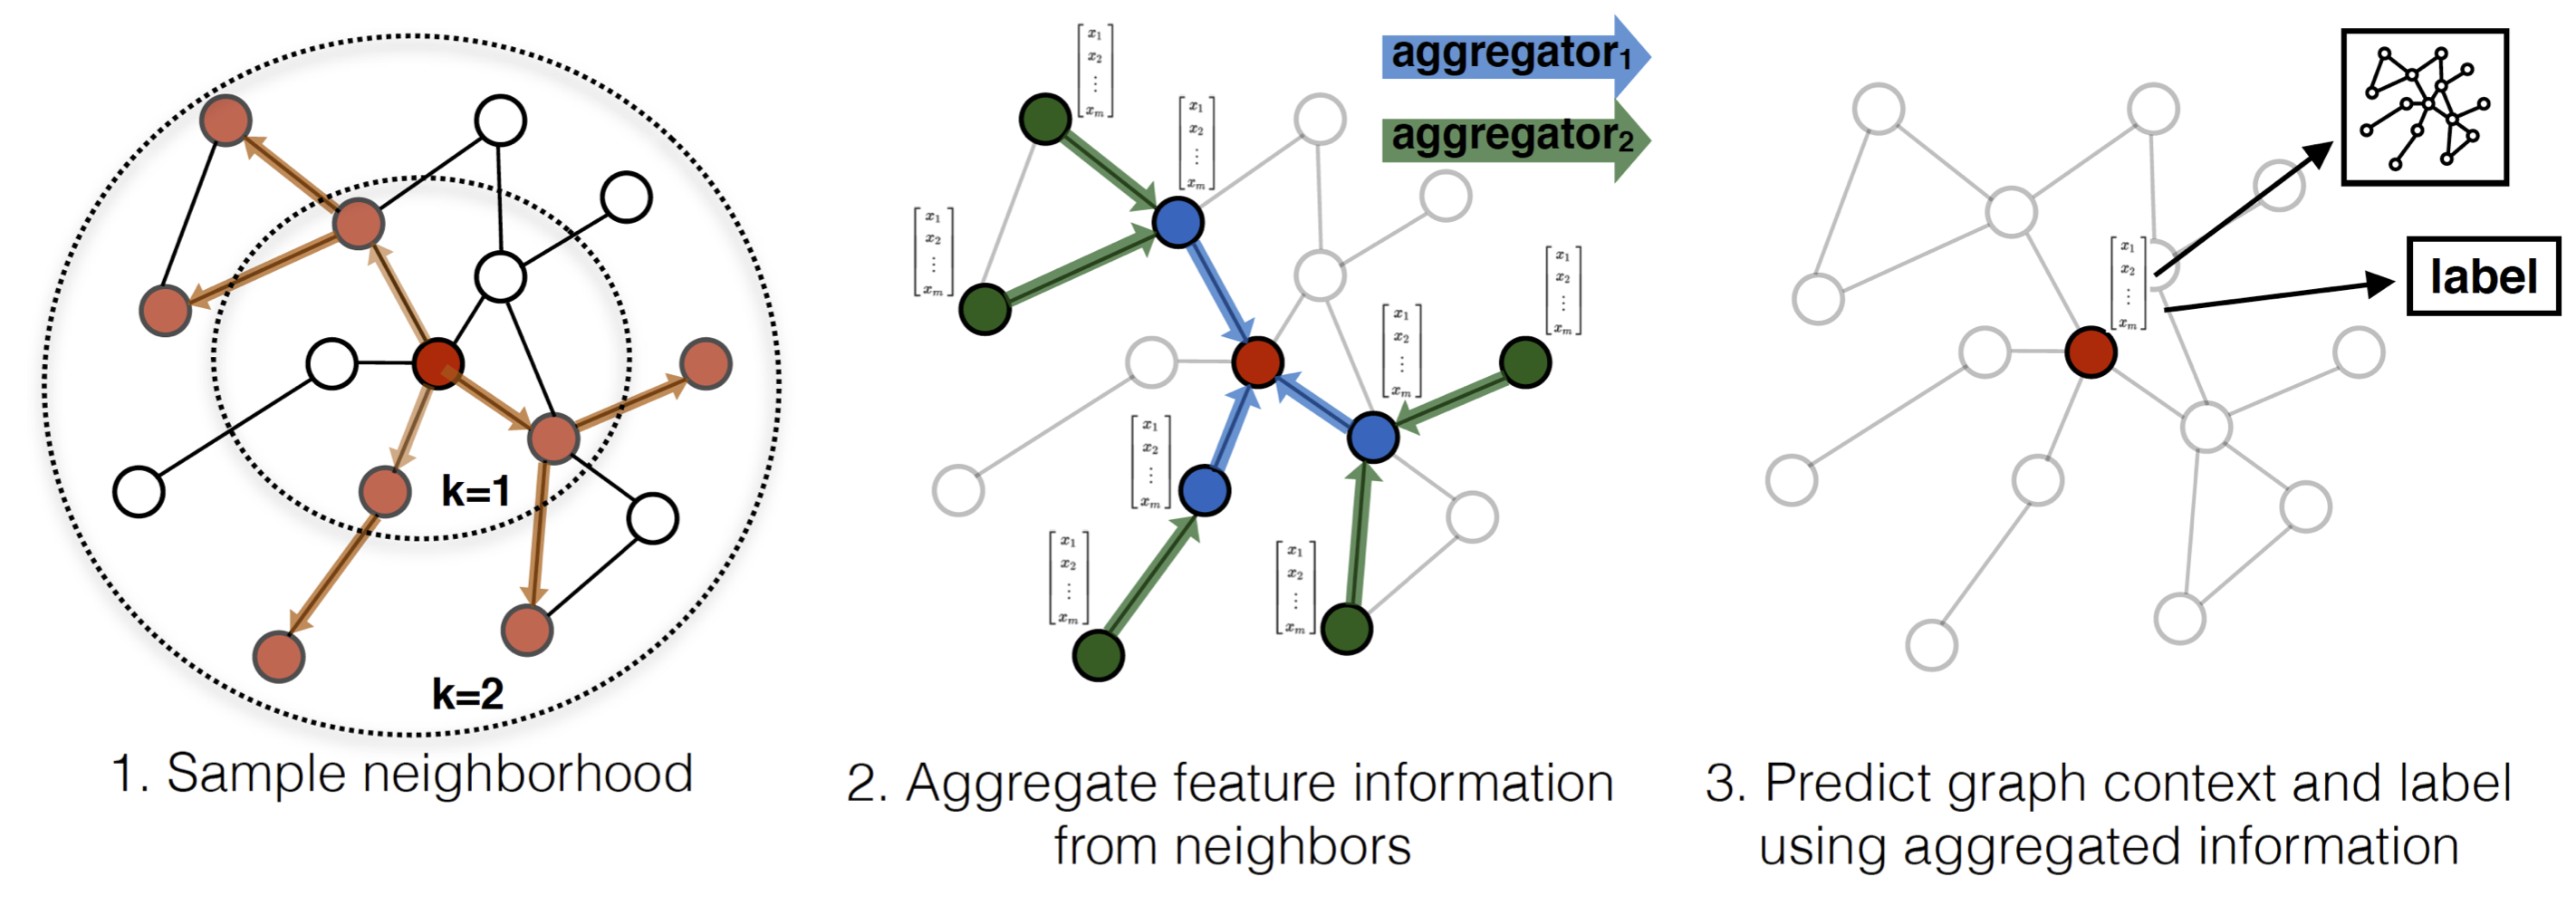
\includegraphics[width=0.8\textwidth]{sample_and_agg.png}
    \caption{Minh họa quy trình lấy mẫu và tổng hợp (Sample and Aggregate) của GraphSAGE}
    \label{fig:sample_and_agg}
\end{figure}

\subsection{Các hàm tổng hợp (Aggregators)}

GraphSAGE hỗ trợ nhiều loại hàm tổng hợp khác nhau, mỗi loại có những đặc điểm riêng:
\begin{itemize}
    \item \textbf{Mean Aggregator:} Tính trung bình cộng các vector đặc trưng của láng giềng. Đây là cách tiếp cận đơn giản và hiệu quả nhất, tương tự như phép tích chập trên đồ thị.
    \item \textbf{Pooling Aggregator:} Đưa các vector láng giềng qua một lớp kết nối đầy đủ (MLP) và thực hiện phép lấy cực đại (element-wise max pooling) để chọn lọc những đặc trưng nổi bật nhất.
    \item \textbf{LSTM Aggregator:} Sử dụng mạng LSTM để tổng hợp thông tin. Tuy nhiên, do LSTM không có tính bất biến với thứ tự (permutation invariant), các láng giềng cần được xáo trộn ngẫu nhiên trước khi đưa vào.
\end{itemize}

Trong đề tài này, hàm \textbf{Mean Aggregator} được ưu tiên sử dụng do tính đơn giản và khả năng tối ưu hóa tốt trên các thiết bị di động có tài nguyên hạn chế.

\section{Device-Cloud Collaborative Learning (DCCL)}

Học tập hợp tác thiết bị - đám mây (Device-Cloud Collaborative Learning - DCCL) là một kiến trúc hiện đại cho phép phân bổ linh hoạt các tác vụ tính toán và lưu trữ giữa máy chủ trung tâm (Cloud) và các thiết bị đầu cuối (Device). Trong bối cảnh hệ thống khuyến nghị, DCCL giải quyết mâu thuẫn giữa nhu cầu về tri thức toàn cục đồ sộ và yêu cầu bảo vệ quyền riêng tư, cá nhân hóa tức thời.

\subsection{Tổng quan kiến trúc}

Kiến trúc DCCL trong đề tài được thiết kế với sự phân định rõ ràng về vai trò của hai thành phần:

\begin{itemize}
    \item \textbf{Phía Đám mây (Cloud Server):}
    \begin{itemize}
        \item Lưu trữ và quản lý đồ thị tương tác toàn cục (Global Graph) bao gồm hàng triệu người dùng và sản phẩm.
        \item Thực hiện các tác vụ tính toán nặng: Huấn luyện mô hình GNN để học các vector nhúng (Global Embeddings).
        \item Cung cấp dịch vụ truy xuất ứng viên (Candidate Retrieval) dựa trên các thuật toán tìm kiếm láng giềng gần nhất (ANN) hoặc duyệt đồ thị.
    \end{itemize}
    \item \textbf{Phía Thiết bị (Device Client):}
    \begin{itemize}
        \item Lưu trữ đồ thị con cục bộ (Local Subgraph) chứa lịch sử tương tác gần nhất của người dùng.
        \item Lưu trữ mô hình ranking thu nhỏ (đã được tối ưu hóa bằng TFLite).
        \item Thực hiện tính toán xếp hạng (Ranking) ngay trên thiết bị để đưa ra kết quả khuyến nghị cuối cùng.
    \end{itemize}
\end{itemize}

\subsection{Ưu điểm của DCCL so với hệ thống truyền thống}

Kiến trúc phối hợp này mang lại nhiều lợi ích vượt trội:

\begin{table}[h!]
    \centering
    \caption{So sánh kiến trúc DCCL và kiến trúc Cloud-centric truyền thống}
    \renewcommand{\arraystretch}{1.5}
    \begin{tabularx}{\textwidth}{|l|X|X|}
        \hline
        \textbf{Tiêu chí} & \textbf{Cloud-centric truyền thống} & \textbf{DCCL (Đề xuất)} \\ \hline
        \textbf{Quyền riêng tư} & Dữ liệu hành vi thô phải đẩy lên Cloud. & Dữ liệu thô lưu tại thiết bị, chỉ truyền vector nhúng. \\ \hline
        \textbf{Băng thông} & Tốn nhiều băng thông để truyền log hành vi. & Tiết kiệm băng thông do chỉ truyền vector nhúng nhỏ gọn. \\ \hline
        \textbf{Độ trễ} & Phụ thuộc vào tốc độ mạng và tải của server. & Suy luận ranking tức thời tại thiết bị. \\ \hline
        \textbf{Cá nhân hóa} & Khó cập nhật sở thích tức thời. & Phản ánh hành vi thời gian thực cực kỳ nhạy bén. \\ \hline
    \end{tabularx}
    \label{tab:dccl_vs_traditional}
\end{table}

\subsection{Luồng inference trong hệ thống DCCL}

Quá trình đưa ra gợi ý cho người dùng trong hệ thống DCCL diễn ra qua các bước sau:

\begin{enumerate}
    \item \textbf{Khởi tạo yêu cầu:} Thiết bị gửi một mã định danh (User ID) lên Cloud khi người dùng bắt đầu phiên làm việc.
    \item \textbf{Truy xuất ứng viên (Cloud):} Đám mây dựa trên tri thức toàn cục để chọn ra một danh sách các sản phẩm tiềm năng (Candidates). Quá trình này thường kết hợp giữa duyệt đồ thị và tìm kiếm độ tương đồng vector.
    \item \textbf{Truyền tải tri thức:} Đám mây gửi danh sách ID ứng viên cùng với các vector nhúng (Item Embeddings) tương ứng về cho thiết bị.
    \item \textbf{Xếp hạng cục bộ (Device):} Thiết bị sử dụng mô hình TFLite để kết hợp Item Embeddings từ Cloud với đặc trưng từ Local Subgraph (lịch sử vừa xem) để tính toán điểm số ranking.
    \item \textbf{Hiển thị kết quả:} Kết quả có điểm số cao nhất được hiển thị tức thời cho người dùng.
\end{enumerate}

\section{Các độ đo và phương pháp đánh giá}

Để đánh giá hiệu quả của mô hình và hệ thống khuyến nghị được đề xuất, dự án tập trung vào hai khía cạnh chính: khả năng dự đoán liên kết của mô hình GNN và khả năng xếp hạng danh sách sản phẩm trên thiết bị.

\subsection{Area Under the ROC Curve (AUROC)}
AUROC đo lường khả năng của mô hình trong việc phân biệt giữa các cặp tương tác thực (positive edges) và các cặp tương tác giả (negative edges). Đây là độ đo cốt lõi được sử dụng trong quá trình huấn luyện và so sánh giữa kiến trúc GraphSAGE và GCN. Giá trị AUROC tiệm cận 1.0 thể hiện mô hình có khả năng dự đoán chính xác sự tồn tại của một liên kết giữa người dùng và sản phẩm.

\subsection{Average Precision (AP)}
AP đánh giá chất lượng của mô hình thông qua việc tính toán diện tích dưới đường cong Precision-Recall. Độ đo này đặc biệt hữu ích trong bài toán khuyến nghị khi chúng ta quan tâm đến việc các sản phẩm liên quan thực sự có được mô hình xếp hạng ở các vị trí cao hay không.
\begin{equation}
    \text{AP} = \sum_n (R_n - R_{n-1}) P_n
\end{equation}

\subsection{Cơ chế xếp hạng Top-K Recommendation}
Trong giai đoạn suy luận trên thiết bị (Inference), sau khi mô hình tính toán điểm số (logits) cho danh sách các sản phẩm ứng viên, hệ thống thực hiện xếp hạng và chỉ trả về $K$ sản phẩm có điểm số cao nhất.
\begin{equation}
    \mathcal{L}_{\text{rec}} = \text{argtopk}_{i \in \mathcal{I}} (\hat{y}_{u,i})
\end{equation}
Trong đó $K$ là số lượng gợi ý hiển thị cho người dùng (mặc định $K=5$ trong hiện thực thực tế của thiết bị). Việc sử dụng Top-K giúp tối ưu hóa không gian hiển thị và giảm tải tính toán cho thiết bị di động.
